\documentclass{report}
\usepackage[margin=1in, paperwidth=8.5in, paperheight=11in]{geometry}
%Math packages%
\usepackage{amsmath}
\usepackage{amsthm}
%Spacing%
\usepackage{setspace}
\onehalfspacing
%Lecture number%
\newcommand{\lectureNum}{8}
%Variables - Date and Course%
\newcommand{\curDate}{January 20, 2017}
\newcommand{\course}{MATH 239}
\newcommand{\instructor}{Luke Postle}
%Defining the example tag%
%\theoremstyle{definition}%
\newtheorem{ex}{Example}[section]
%Setting counter given the lecture number%
\setcounter{chapter}{\lectureNum{}}
%Package for drawing graphs%
\usepackage{tikz}
\usepackage{verbatim}
\usetikzlibrary{arrows}

\begin{document}
%Note title%
\begin{center}
\begin{Large}
\textsc{\course{} | Lecture \lectureNum{}}
\end{Large}
\end{center} 
\noindent \textit{Bartosz Antczak} \hfill
\textit{Instructor: \instructor{}} \hfill
\textit{\curDate{}}
\rule{\textwidth}{0.4pt}

% Actual Notes%
\subsubsection{Review of last lecture}
We spoke about \textit{leaves}. A leaf is a vertex of degree 1. We also covered some important theorems on trees, forests, and leaves:
\subsubsection{Theorem 1}
\begin{center}
\textit{If $G$ has a minimum degree of at least 2, then $G$ contains a cycle}
\end{center}
\subsubsection{Theorem 2}
\begin{center}
\textit{If $T$ is a tree and $v$ is a leaf of $T$, then $T-v$ is a tree}
\end{center}
\subsubsection{Theorem 3}
\begin{center}
\textit{If $T$ is a tree, then $\vert E(G)\vert = \vert V(G) \vert -1$}
\end{center}
\section{Additional Theorems involving Trees}
\subsection{Corollary 1}
\begin{center}
\textit{If $T$ is a  tree on $n$ vertices, then}
$$\sum_{v \in T} \mathrm{deg}(v) = 2 \vert E(T) \vert = 2(n-1) = 2n - 2$$
\end{center}
(We have $2(n-1)$ because a tree on $n$ vertices will have $n-1$ edges, as proven in Theorem 3). Now, we can rewrite this as
$$\sum_{v\in T} (\mathrm{deg}(v) - 2) = \sum_{v\in T} \mathrm{deg}(v) -2n = -2$$
Let $d_i$ denote the number of vertices of degree $i$. This results in the sum on the left side being equal to
\begin{align*}
\sum_{v\in T} (\mathrm{deg}(v) - 2) &= \sum_{v\in T} \mathrm{deg}(v) - 2n\\
&= \sum_{i=1}^n id_i - 2\sum_{i=1}^n d_i \\
&= \sum_{i=1}^n (i-2)d_i
\end{align*}
Which means that we have:
$$\sum_{i=1}^n (i-2)d_i = -d_1 + 0d_2 + 1d_3 + 2d_4 + \cdots = -2$$
\subsection{Lemma 1}
\begin{center}
\textit{If $T$ is a tree on at least 2 vertices, then}
\end{center}
$$d_1 = 2 + d_3 + 2d_4 + \cdots = 2 + \sum_{i=3}^n d_i$$
This equation stems from our calculations in corollary 1.
\section{Spanning}
\subsubsection{Definition}
A subgraph $H$ of graph $G$ is \textbf{spanning} if $V(H) = V(G)$.\\
A \textbf{spanning tree} $T$ of a graph $G$ is a tree $T$ that is a subgraph of $G$ such that $V(G) = V(T)$. 
%(A vertex is a tree, called a ``bush").
\begin{ex}
Consider $K_4$. Observe that the two adjacent graphs are spanning trees of $K_4$
\end{ex}
%K_4 Graph%
\begin{center}
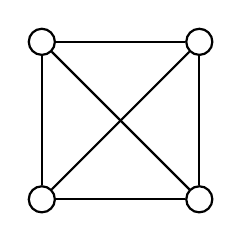
\begin{tikzpicture}[-,auto,node distance=2cm,
                    thick,main node/.style={circle, draw,font=\sffamily\small}]

  %Square%
  \node[main node] (4) []{};
  \node[main node] (5) [below of=4]{};
  \node[main node] (6) [right of=5]{};
  \node[main node] (7) [above of=6]{};
  
  \path[every node/.style={font=\sffamily\small}]
    %Square%
    (4) edge node [right] {} (7)
        edge node [right] {} (5)
        edge node [right] {} (6)
    (6) edge node [right] {} (5)
        edge node [right] {} (7)
    (5) edge node [right] {} (7);
\end{tikzpicture}
$\qquad\qquad\qquad$
%P_4%
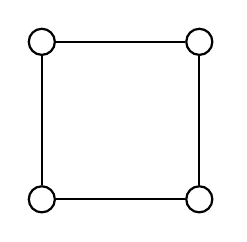
\begin{tikzpicture}[-,auto,node distance=2cm,
                    thick,main node/.style={circle, draw,font=\sffamily\small}]

  %Square%
  \node[main node] (4) []{};
  \node[main node] (5) [below of=4]{};
  \node[main node] (6) [right of=5]{};
  \node[main node] (7) [above of=6]{};
  
  \path[every node/.style={font=\sffamily\small}]
    %Square%
    (4) edge node [right] {} (5)
    	edge (7)
    (6) edge node [right] {} (7)
    (5) edge node [right] {} (6);
\end{tikzpicture}
$\qquad$
%Other graph%
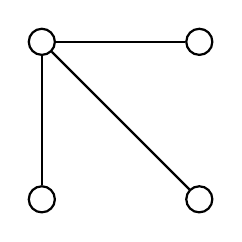
\begin{tikzpicture}[-,auto,node distance=2cm,
                    thick,main node/.style={circle, draw,font=\sffamily\small}]

  %Square%
  \node[main node] (4) []{};
  \node[main node] (5) [below of=4]{};
  \node[main node] (6) [right of=5]{};
  \node[main node] (7) [above of=6]{};
  
  \path[every node/.style={font=\sffamily\small}]
    %Square%
    (4) edge node [right] {} (7)
        edge node [right] {} (5)
        edge node [right] {} (6);
\end{tikzpicture}
\end{center}
Generally, there are a lot of spanning trees for every graph.\\
A natural question that arises from studying spanning trees is \textit{which graphs have a spanning tree?} Well, for such a graph $G$, we know that the spanning tree $T$ will contain all of the same vertices as $G$, and since $T$ is a tree, it must be connected, hence we know that $G$ will be connected as well. This observation raises the question
\begin{center}
\textit{Does every connected graph have a spanning tree?}
\end{center}
The answer is yes! We will prove it in the following theorem.
\subsubsection{Theorem 8.1.1}
\begin{center}
\textit{Graph $G$ is connected if and only if $G$ has a spanning tree}
\end{center}
\textbf{Proof of Theorem 8.1.1:}
\begin{itemize}
\item Proof of $\impliedby$: \textit{If $G$ has a spanning tree, then $G$ is connected}\\
Let $T$ be a spanning tree of $G$, and $x,y \in V(G)$. Since $T$ is spanning, $x,y\in V(T)$. Since $T$ is connected (by definition), there exists a path $P$ from $x$ to $y$ in $T$. Since $T$ is a subgraph of $G$, there exists a path $P$ from $x$ to $y$ in $G$, which implies that $G$ is connected as desired.
\item 
Proof of $\implies$: \textit{If $G$ is connected, then $G$ has a spanning tree}\\
Let $H$ be a connected spanning subgraph of $G$ and subject to that, $\vert E(H) \vert$ is minimized (i.e., find such a connected subgraph $H$ in $G$ that contains the least number of edges). Note that $H$ \underline{exists} since $G$ is a connected spanning subgraph of itself.
\newpage From here, I claim that $H$ is a tree. We already showed $H$ is connected, so all we have to prove is that $H$ doesn't contain a cycle (we'll do so by contradiction):\\
Suppose not. By our assumption, $H$ is connected, so if $H$ is not a tree, then $H$ contains a cycle. Let $C$ be a cycle of $H$ and let $e \in E(C)$. Let $H^\prime = H-e$. Note that $H^\prime$ is spanning because $V(H^\prime) = V(H) = V(G)$. We claim that $H^\prime$ is connected. To see this, let $x,y \in V(H^\prime)$. But then $x,y \in V(H)$. Since $H$ is connected, then there exists a path $P$ from $x$ to $y$ in $H$.\\
Now, if $e \not\in E(P)$, then $P$ is a path in $H^\prime$ as desired.\\
If $e \in E(P)$, let $W = P-e + (E(C) - e)$. Then $W$ is a walk in $H^\prime$ from $x$ to $y$. So by theorem, there exists a path in $H^\prime$ from $x$ to $y$, thus $H^\prime$ is connected as claimed. BUT then, $\vert E(H^\prime) \vert = \vert E(H) \vert - 1$, which contradicts the minimality of $H$. This proves the claim of $H$ being a tree and hence a spanning tree as desired.

\end{itemize}
\subsubsection{Corollary of Theorem 8.1.1}
\begin{center}
\textit{Let $G$ be a connected graph. $\vert E(G) \vert = \vert V(G)\vert - 1$ if and only if $G$ is a tree}
\end{center}
\textbf{Proof of Corollary:}\\
\begin{itemize}
\item Proof of $\impliedby$: \textit{if $G$ is a tree, then $\vert E(G)\vert = \vert V(G)\vert - 1$}\\
We proved this in the last lecture ;)
\item Proof of $\implies$: \textit{if $\vert E(G)\vert = \vert V(G)\vert - 1$, then $G$ is a tree}\\
Suppose $\vert E(G)\vert = \vert V(G)\vert - 1$. By theorem, if $G$ is connected, $G$ has a spanning tree $T$. Since $T$ is a tree, $\vert E(T)\vert = \vert V(T)\vert - 1$. Since $T$ is spanning, $V(T) = V(G)$. Thus, $\vert E(T)\vert = \vert V(G)\vert - 1$. Yet by supposition, $\vert E(G)\vert = \vert V(G)\vert - 1$. Thus, since $T$ is a subgraph of $G$, $T$ and $G$ have the same edges! But since $T$ is spanning, $T$ and $G$ also have the same vertices! Thus, $T = G$, hence $G$ is a tree as desired.
\end{itemize}

\subsection{Algorithm to Decide if a Graph is Connected}
Let G be a graph
\begin{enumerate}
\item Pick $v \in V(G)$. Let T = v
\item While $\delta(V(T)) \neq \emptyset$; let $e \in \delta(V(T))$. Set $T = T +e$ 
\item If $V(T) = V(G)$, then $T$ is a spanning tree. If not, then let $X = V(T)$ and realize that $\delta(X)$ is empty!
\end{enumerate}
%END%
\end{document}